\documentclass{beamer}	
\mode<presentation>
 
\usepackage{pdfpages}
\usepackage{fancyvrb}
\usepackage{chemarr}

\usepackage{amsmath}		%% mathematics typesetting
\usepackage{amssymb}
 
\usepackage{epigraph}   %% nice setting of quotations

\usepackage{tabularx} %% allows to use row colours in tables

\usepackage{ulem}

\usepackage{booktabs}

\usepackage{siunitx} %% tpyeset SI units

\usepackage{CJKutf8} %% typeset Chinese characters

\usepackage{pdfpages}%% include pdfs

\usepackage{graphicx}
\usepackage{animate} %% show animated gifs

\DeclareMathAlphabet{\mathcalligra}{T1}{calligra}{m}{n}


% Color and Theme. Can be changed. However, this one's quite nice.
\usetheme{Madrid}
\definecolor{theme}{rgb}{0.84,0,0.21}
\usecolortheme[named=theme]{structure}

%%  Title information
\title[M11.13.1 Psychophysik]{M11.13.1 Psychophysik: \\ Allgemeine Sinneswahrnehmung}
\author[melanie.stefan@medicalschool-berlin.de]{}
\institute[]{Prof. Melanie Stefan \\ melanie.stefan@medcialschool-berlin.de}
\date{WiSe 2022/23}
 

% Table of contents to pop up at the beginning of each section
\AtBeginSection[]
{
  \begin{frame}<beamer>
    \frametitle{Outline}
    \tableofcontents[currentsection,currentsubsection]
  \end{frame}
}
 
\beamertemplatenavigationsymbolsempty

\begin{document}


{ \usebackgroundtemplate{
\includegraphics[width=1.2\paperwidth]{MSB_Titelseite.pdf}} 
\begin{frame}

 \maketitle 

$\,$\\[6cm] 


\end{frame} 
}


%% Hook:

{ \usebackgroundtemplate{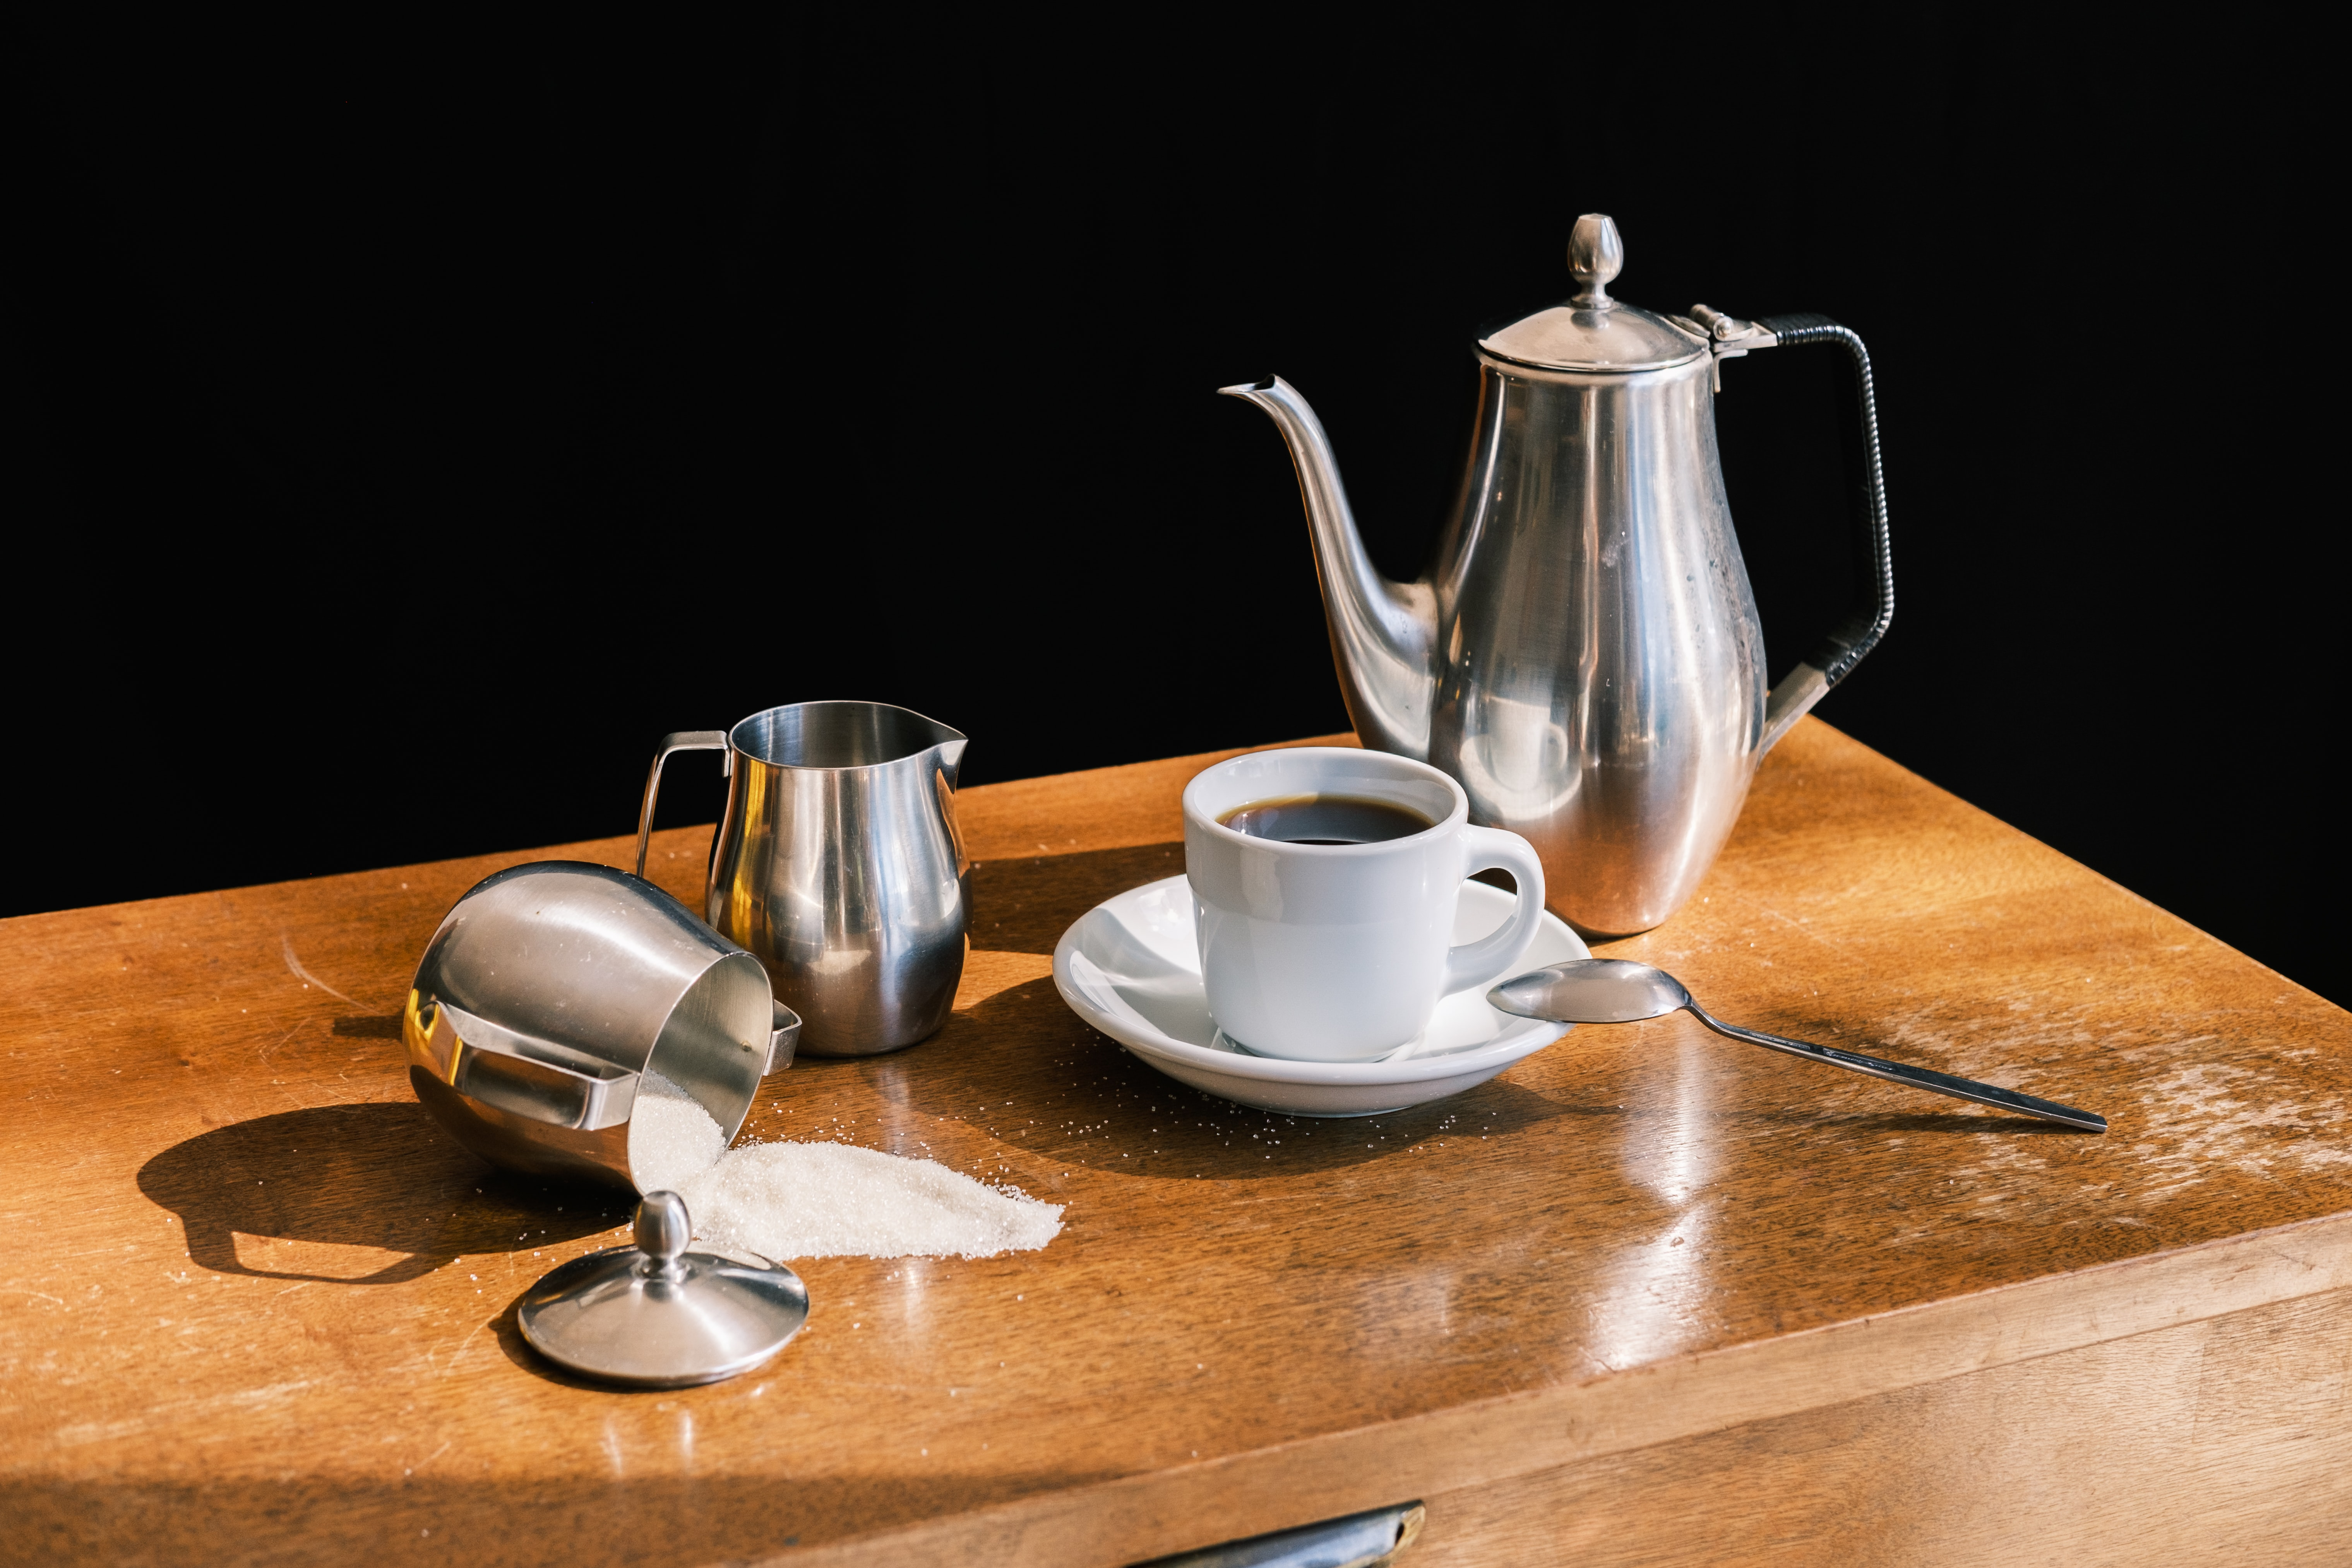
\includegraphics[width=1.2\paperwidth]{still_life.jpg}} 
\begin{frame}
\textcolor{white}{Wir nehmen die Welt durch unsere Sinne wahr \dots}

$\,$\\[3.5cm]

\pause
\textcolor{white}{Aber wie?}

$\,$\\[4cm]

\end{frame}
}

 
% %% %% TLIA
\begin{frame}{In diesem Semester geht es um Sinnesphysiologie}

Vorlesungen im 4. Semester:

\begin{itemize}
\item
Allgemeine Sinnesphysiologie 
\begin{itemize}
    \item Psychophysik und allgemeine Sinnesphysiologie
\end{itemize}
\item
Somatosensorik 
\begin{itemize}
    \item Somatosensorik 1: Tastsinn
    \item Somatosensorik 2: Propriozeption und Thermorezeption
    \item Somatosensorik 3: Nozizeption und Schmerz
\end{itemize} 
\item Visuelles System 
    \begin{itemize}
    \item
    Visuelles System 1: Dioptrischer Apparat 
    \item
    Visuelles System 2: Retinale Signalverarbeitung, zentrale Sehbahn 
    \end{itemize}
\item
Gehör und Gleichgewicht 
\begin{itemize}
    \item Auditorisches System: Hören und periphere Hörbahnen 
    \item Vestibuläres System
    
\end{itemize}
\item     Chemische Sinne
\begin{itemize}
    \item 
    Chemosensorik: Geschmack und Geruch
\end{itemize}
    
\end{itemize}


(Der Rest sind Repetitorien)

\end{frame}

\begin{frame}{In diesem Semester geht es um Sinnesphysiologie}

Vorlesungen im 4. Semester:

\begin{itemize}
\item
Allgemeine Sinnesphysiologie 
\begin{itemize}
    \item \textcolor{theme}{Psychophysik und allgemeine Sinnesphysiologie}
\end{itemize}
\item
Somatosensorik 
\begin{itemize}
    \item Somatosensorik 1: Tastsinn
    \item Somatosensorik 2: Propriozeption und Thermorezeption
    \item Somatosensorik 3: Nozizeption und Schmerz
\end{itemize} 
\item Visuelles System 
    \begin{itemize}
    \item
    Visuelles System 1: Dioptrischer Apparat 
    \item
    Visuelles System 2: Retinale Signalverarbeitung, zentrale Sehbahn 
    \end{itemize}
\item
Gehör und Gleichgewicht 
\begin{itemize}
    \item Auditorisches System: Hören und periphere Hörbahnen 
    \item Vestibuläres System
    
\end{itemize}
\item     Chemische Sinne
\begin{itemize}
    \item 
    Chemosensorik: Geschmack und Geruch
\end{itemize}
    
\end{itemize}


(Der Rest sind Repetitorien)

\end{frame}



%  % Learning Objectives
 
\begin{frame}

 \frametitle{Nach dieser Vorlesung sollten Sie folgendes können}



\begin{block}{Grundlagen:}




\begin{itemize}

    \item 
Die Begriffe Modalität, Qualität und Intensität erklären
    \item 
Erklären, was eine Schwellenbestimmung ist 
    \item 
Die Gesetze von Weber/Fechner und Stevens anführen und anwenden
    \item 
Adäquate Reize definieren
    \item 
Den allgemeinen Weg der Wahrnehmung vom Reiz zu den entsprechenden Zentren im Gehirn erläutern 
    \item 
Effekte von neuronalen Netzwerken auf die Reizwahrnehmung erklären
\end{itemize}


\end{block}



 

\begin{block}{Klinik:}

\begin{itemize}
    
\item 
Methoden zur Bestimmung von Schwellen erläutern 
\item
Agnosie erklären und ein Beispiel geben
\item
Synästhesie erklären und ein Beispiel geben


\end{itemize}


\end{block}



\end{frame}



%% %% %% Main Body
 

\section{Was nehmen wir wahr?}

%% Modalität, Intensität, Qualtiät

%% Adäquater Reiz oder nicht, Gesetz der spezifischen Sinnesenergien - Synästheie


\section{Wie nehmen wir es wahr?}

%% Wahrnehmungsbahn allgemein

%% Arten von Rezeptoren, Generatorpotential

%% Transduktion, Transmission

%% Frequenzkodierung

%% Rezeptive Felder

%% Netzwerk-Effekte: Konvergenz, Divergenz, Laterale Hemmung, Bsp. Kontrastwahrnehmung, rekurrente Hemmung


%% Sensorische Bahnen

%% Rolle von Erfahrung, Bsp. Agnosie, Bsp. The dress

%% Aufmerksamkeit, Bsp. Gorilla 


\section{Woher wissen wir das?}

%% Reizschwellen
%% Bestimmung von Reizschwellen - incld. 2AFC

%% Weber-Fechner
%% Stevens



%% %% %% %% Review



\begin{frame}

 \frametitle{Jetzt* sollten Sie folgendes können}



\begin{block}{Grundlagen:}




\begin{itemize}

    \item 
Die Begriffe Modalität, Qualität und Intensität erklären
    \item 
Erklären, was eine Schwellenbestimmung ist 
    \item 
Die Gesetze von Weber/Fechner und Stevens anführen und anwenden
    \item 
Adäquate Reize definieren
    \item 
Den allgemeinen Weg der Wahrnehmung vom Reiz zu den entsprechenden Zentren im Gehirn erläutern 
    \item 
Effekte von neuronalen Netzwerken auf die Reizwahrnehmung erklären
\end{itemize}


\end{block}



 

\begin{block}{Klinik:}

\begin{itemize}
    
\item 
Methoden zur Bestimmung von Schwellen erläutern 
\item
Agnosie erklären und ein Beispiel geben
\item
Synästhesie erklären und ein Beispiel geben


\end{itemize}


\end{block}



\end{frame}




%% %% %% %% Feedbackhinweisblock

\begin{frame}
\frametitle{Danke für Ihr Feedback!}

\begin{columns}[c]

\begin{column}{6cm}
\begin{center}
 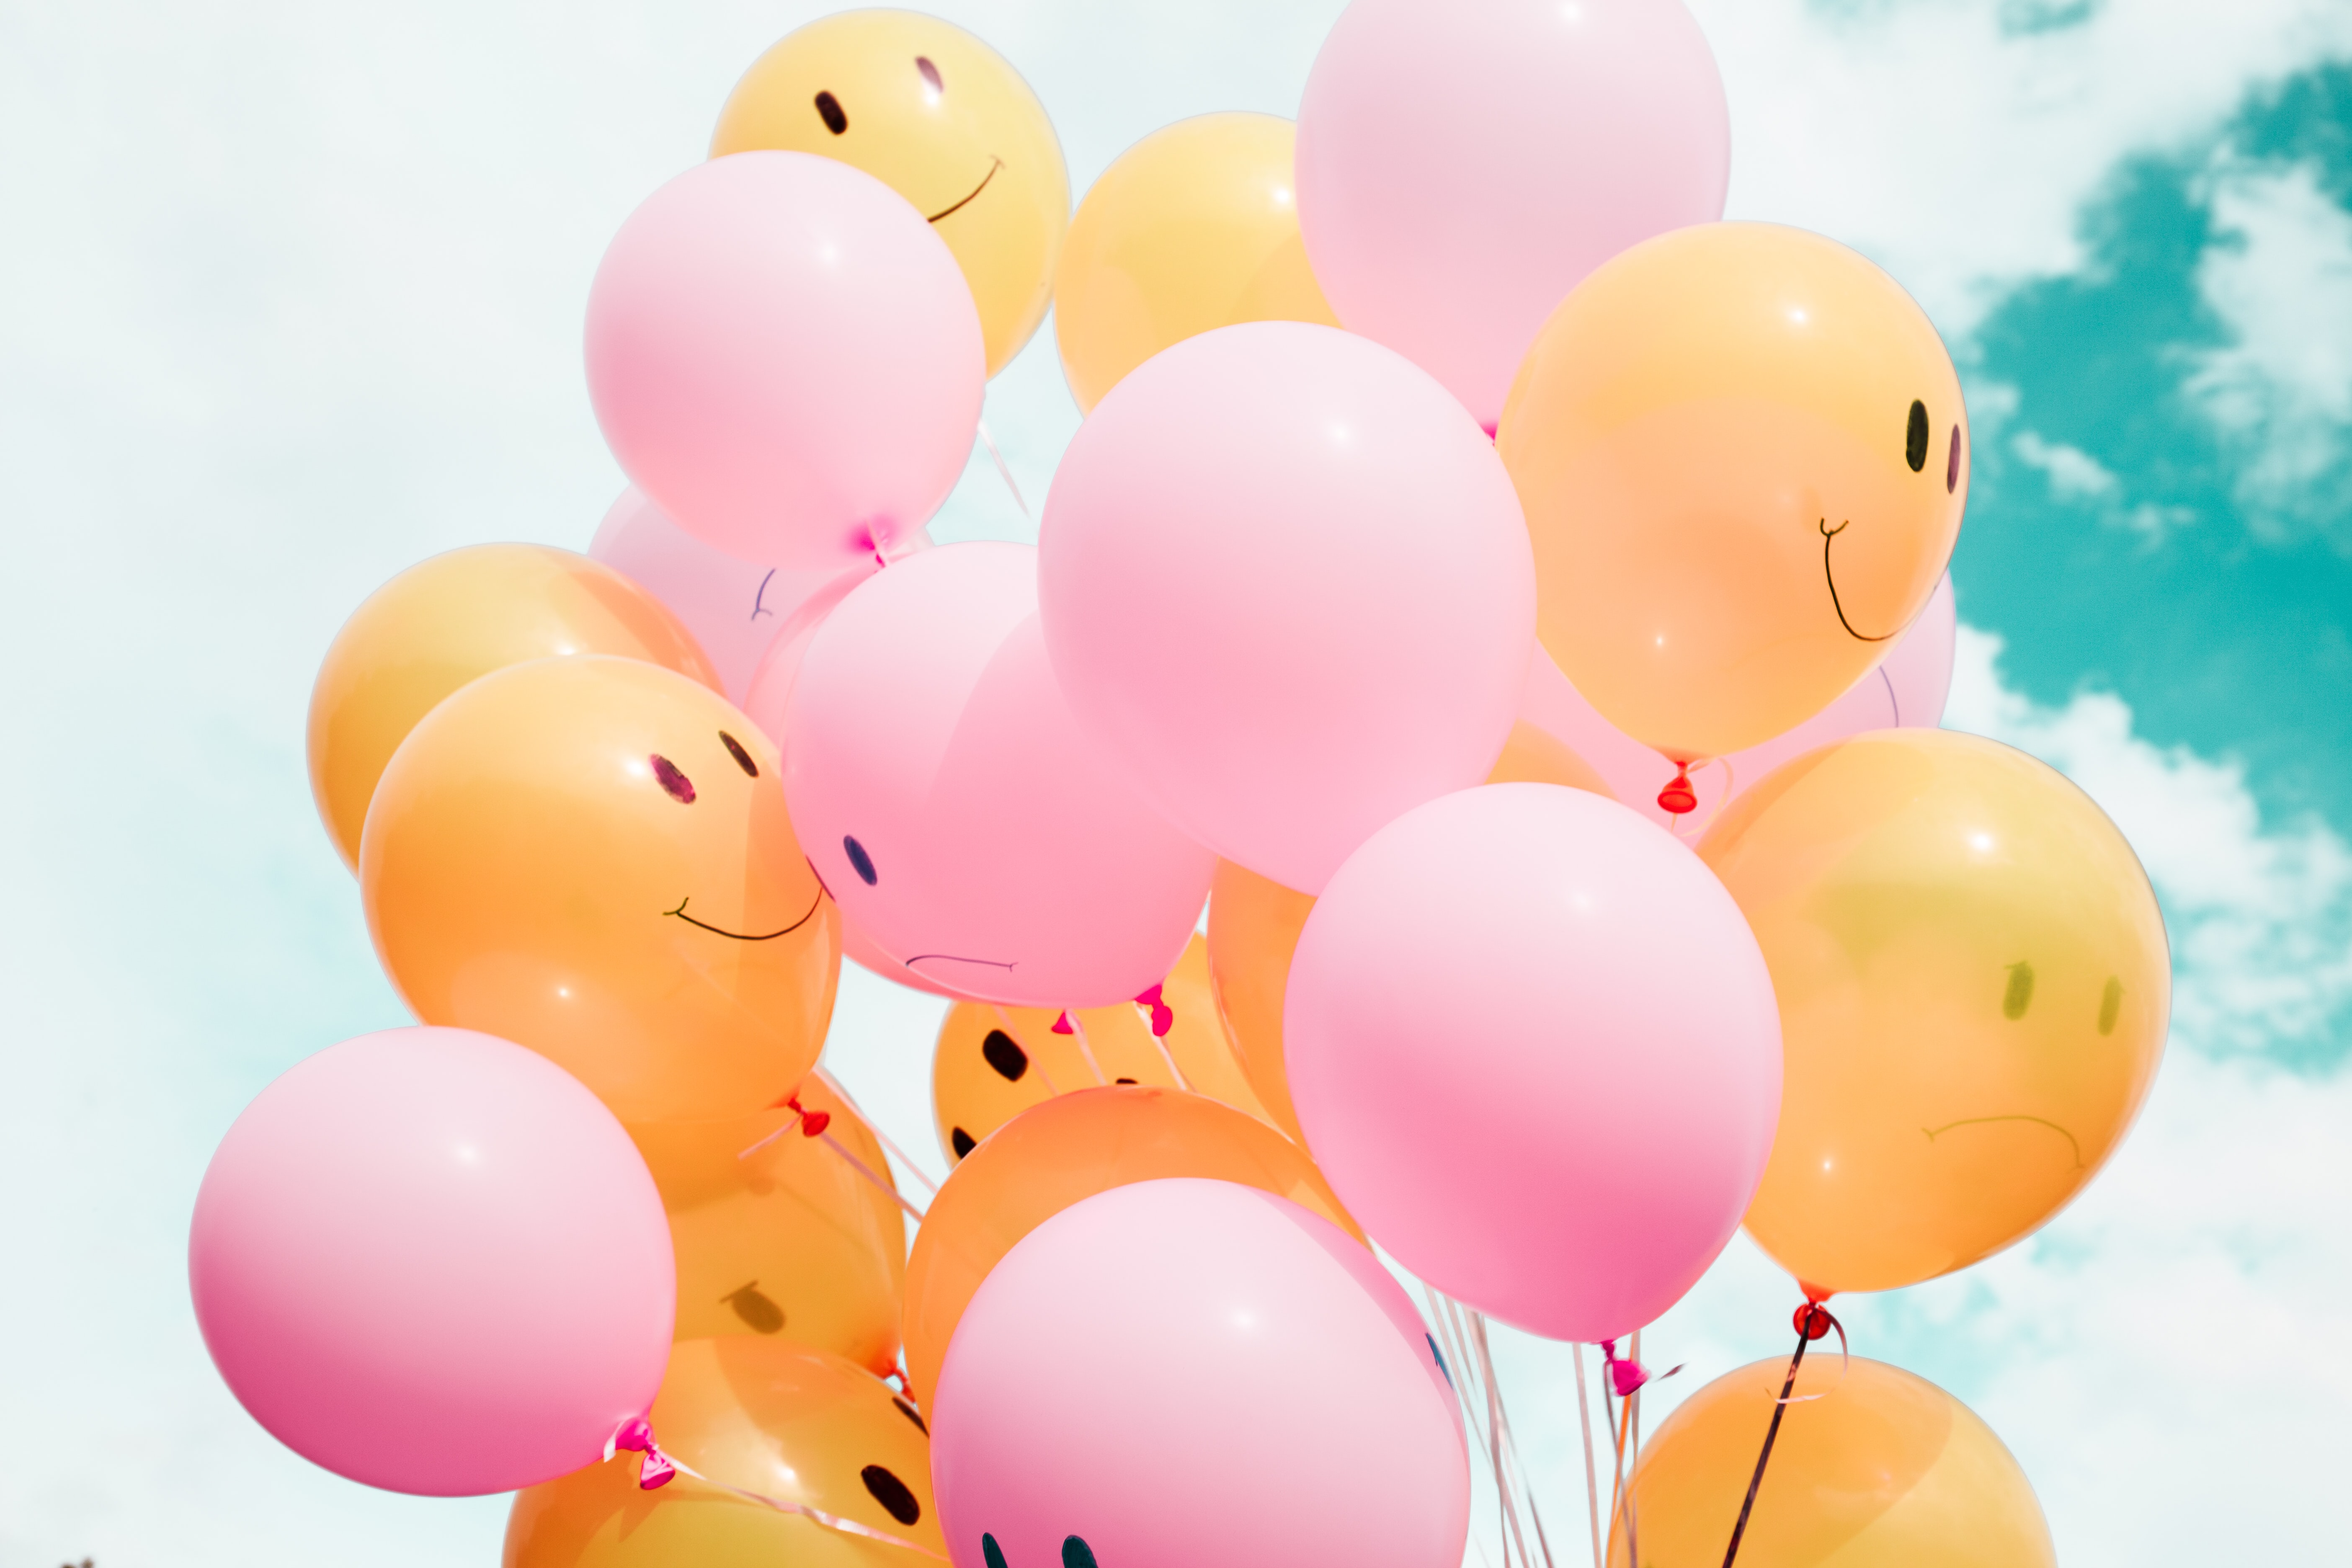
\includegraphics[width=\textwidth]{smilie_balloons.jpg}
\end{center}

\end{column}

\begin{column}{4cm}


\begin{center}

\includegraphics[width=\textwidth]{feedback_QR.png}
\end{center}
\end{column}


\end{columns}
\end{frame}




%% %% %% Bildnachweis
\begin{frame}
\frametitle{Bildnachweis}
\begin{tiny}



 
\begin{itemize}

\item
Luftballons mit frohen und traurigen Smileys. Photo by \href{https://unsplash.com/@artbyhybrid?utm_source=unsplash&utm_medium=referral&utm_content=creditCopyText}{Hybrid} on \href{https://unsplash.com/s/photos/feedback?utm_source=unsplash&utm_medium=referral&utm_content=creditCopyText}{Unsplash}


\item
Stillleben mit Kaffee. Photo by \href{https://unsplash.com/@garrethpb?utm_source=unsplash&utm_medium=referral&utm_content=creditCopyText}{Garreth Paul} on \href{https://unsplash.com/s/photos/still-life?utm_source=unsplash&utm_medium=referral&utm_content=creditCopyText}{Unsplash}
  
\end{itemize}
\end{tiny}
\end{frame}






\end{document}

%%% Frequently used snippets

%% \begin{columns}[c]

%% \begin{column}{5cm}
%% \end{column}

%% \begin{column}{5cm}
%% \end{column}


%% \end{columns}




